\documentclass[lettersize,journal,12pt,conference]{IEEEtran}
\usepackage{fontspec}
\usepackage{amsmath,amsfonts}
\usepackage{algorithmic}
\usepackage{algorithm}
\usepackage{array}
\usepackage[caption=false,font=normalsize,labelfont=sf,textfont=sf]{subfig}
\usepackage{textcomp}
\usepackage{stfloats}
\usepackage{url}
\usepackage{verbatim}
\usepackage{xeCJK}
\usepackage{lettrine}
\usepackage{graphicx}
\usepackage{titling}
\usepackage{titlesec}
\usepackage{balance}
\usepackage{textcase}
\usepackage{setspace}
\usepackage[justification=centering]{caption}
\setmainfont{Times New Roman}[SmallCapsFont=TeX Gyre Termes:+smcp]
\newenvironment*{proof}{{\noindent\it Proof}\quad}

% rule to break words
\hyphenation{}
\def\BibTeX{{\rm B\kern-.05em{\sc i\kern-.025em b}\kern-.08em
T\kern-.1667em\lower.7ex\hbox{E}\kern-.125emX}}
\pretitle{\begin{center}\fontsize{16}{18}\selectfont\bfseries}
\posttitle{\end{center}}
\preauthor{\begin{center}\fontsize{10}{12}\selectfont}
\postauthor{\end{center}}
\predate{\begin{center}\fontsize{10}{12}\selectfont}
\postdate{\end{center}}
\titleformat{\section}
{\filcenter\fontsize{14}{16}\bfseries\uppercase}
{\thesection}
{1em}
{}
\renewenvironment{abstract}
{\fontsize{12}{14}\textit{\textbf{\abstractname---}}\bfseries\ignorespaces}
{}
\renewenvironment{IEEEkeywords}
{\fontsize{12}{14}\textit{\textbf{Keywords---}}\bfseries\ignorespaces}{}
\begin{document}
\onehalfspacing
\title{Unveiling the PageRank Algorithm: Principles, Performance, and Enhancements}
\author{Wu Zelin, Wu Zekai, Li Pengda}

\maketitle\thispagestyle{headings}
\markboth{10225101428 吴泽霖\quad10225101429 武泽恺\quad10225101460 李鹏达}{}

\begin{abstract}
	This paper introduces the PageRank algorithm, which is a fundamental algorithm in web search. After an introduction to the background of the PageRank algorithm and several related works, we present the foundational principles and implementation of the PageRank algorithm. Then, we analyze its performance by experiments and test the impact of the factors that can influence the search results and page rankings, especially the damping factor. Ultimately, we discuss the existing flaws and potential enhancements, exploring the approaches to improve PageRank performance.
\end{abstract}

\begin{IEEEkeywords}
	PageRank, Search Engine, Matrix
\end{IEEEkeywords}


\section{Introduction}

\subsection{Research Background}

\lettrine{W}{ith} 
the proliferation of the Internet technology, the explosively increasing number of web pages on the World Wide Web has created the demand for the web searching engines with high-efficiency and high-effectiveness. 
For the biggest search engine company Google, which held a global market share of 91.54\% until November 2023\footnote[1]{Search Engine Market Share Worldwide, Statcounter GlobalStats, 2023, https:
	//gs.statcounter.com/search-engine-market-share}, it is of primary significance to develop a powerful search algorithm to provide users with the most relevant and useful results in the shortest time.

\begin{figure}[h]
	\centering
	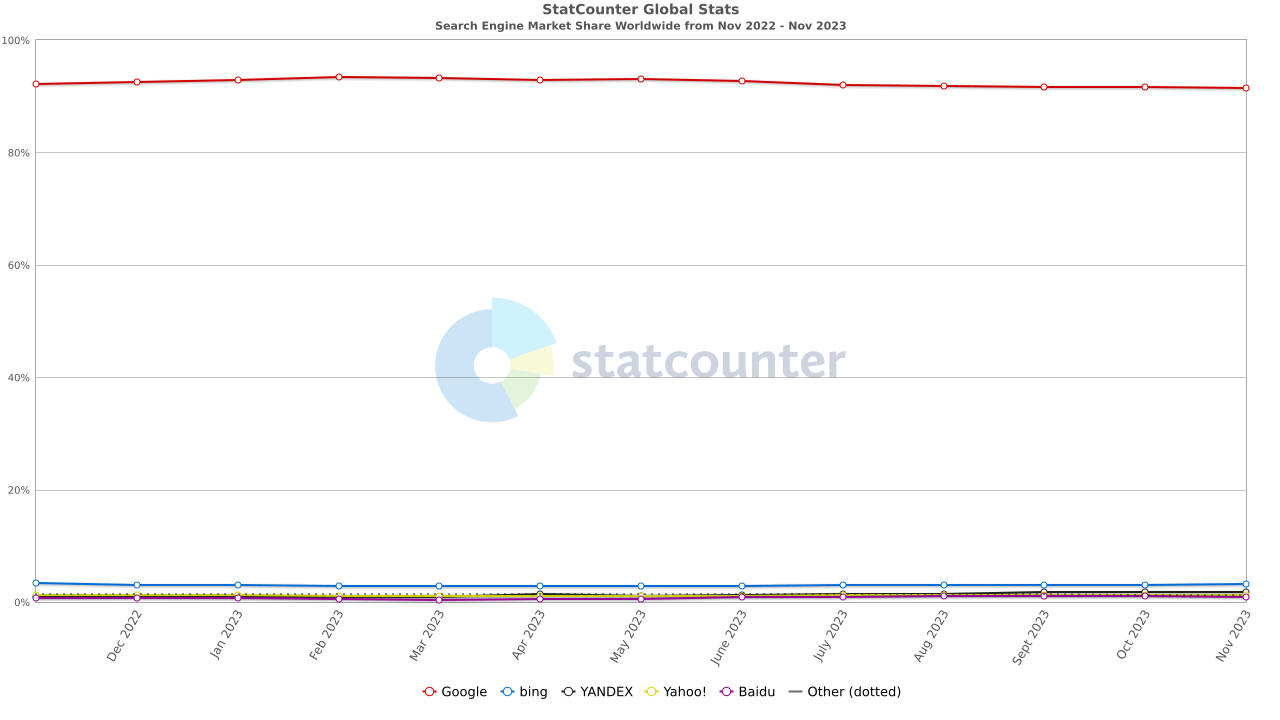
\includegraphics[width=2.5in]{images/fig2.png}
	\caption{Google's market share in the global search engine market from December 2022 to November 2023.}
	\label{fig1}
\end{figure}

Previous studies on web searching algorithms have proven that keyword matching algorithm\cite{ref1}, vector space model\cite{ref2}, and the Hyperlink-Induced Topic Search algorithm(HITS)\cite{ref3} were useful, efficient and effective in the early days of the Internet.

However, these algorithms have been unable to meet the growing demand of users. The users' search queries are becoming diversified and the web pages are becoming complex. 
According to the statistics, the number of web pages, a 130-fold increase over 20 years, has surged to 130 trillion in 2016, which means it takes much longer time to search for the most relevant web pages.
Besides, they only take into account the page content but ignore the graphical structure of the web pages.
To overcome the aformentioned chanllenge, Google has developed a state-of-the-art algorithm called PageRank, which is currently a fundamental algorithm in web search, redefining how we navigate web search.

\subsection{Origin of the PageRank Algorithm} 

PageRank is an algorithm developed by Larry Page and Sergey Brin in the late 1990s to measure the importance of web pages.
Originally created for the Google search engine, it is named after one of the founder of Google Larry Page. Except for the searching use, the Google search engine also takes advantage of this algorithm to analyze the relevance and importance of web pages, considering it as one of the factors to evaluate the effectiveness of web page optimization.

\subsection{Outline of this Paper}

In this paper, we present the following insights and research:
\begin{itemize}
	\item The foundational principles and implementation of the PageRank algorithm.(Section 3, Subsection A)
	\item Analysis of its performance and the impact of the factors that can influence the search results and page rankings.(Section 4, Subsection A)
	\item Discussion on potential enhancements and exploration of the possibility of other factors that can improve PageRank performance.(Section 5, Subsection A and B)
\end{itemize}

In the next section, we introduce the preliminaries and the related work of the PageRank algorithm.

\section{Related Work}

This section shows the brief concept and preliminaries of the PageRank algorithm, which is indispensable for the understanding of the following sections.

%这里需要改,改成之前的算法介绍,不要用这个
\subsection{Hyperlink-Induced Topic Search algorithm}

The Hyperlink-Induced Topic Search (HITS) algorithm is a link analysis algorithm that ranks web pages, developed by Jon Kleinberg. This algorithm assigns two scores to each page,including hub score and authority score. Hub is a web page that link to many other web pages, while authority is a web page that is linked by many hubs. This algorithm computes the hub and authority scores for every page on the World Wide Web. The hub and authority scores are computed iteratively until the ultimate structure of web pages is formed. This algorithm has been applied to many search engines, computational biology and many other fields. 

However, its limitations are exposed in many circumstances. For instance, simply classifying the web pages into two categories, it is unable to rank the web pages in a more precise way, which worsens as the number of web pages increases. To address this problem, the PageRank algorithm introduces link weights to define the importance of a hyperlink. For instance, if a web page is linked by an important web page, then its importance will also be higher.

For the large searching engine, simplicity and efficiency are significant considerations. The HITS algorithm requires multiple iterative and complex calculations, leading to its unsuitability for the current need.

\subsection{Synopsis of PageRank}

PageRank is a link analysis algorithm\cite{ref4}. It assigns a numerical weighting to each web page of all hyperlinked web pages. We call the weight value of any element E as ``PageRank of E", which is represented as symbol $\boldsymbol{PR(E)}$. 
The weight value of a web page could be affected by other factors, such as "Author Rank," which takes into account the author's reputation and authority.

\begin{figure}[h]
    \centering
    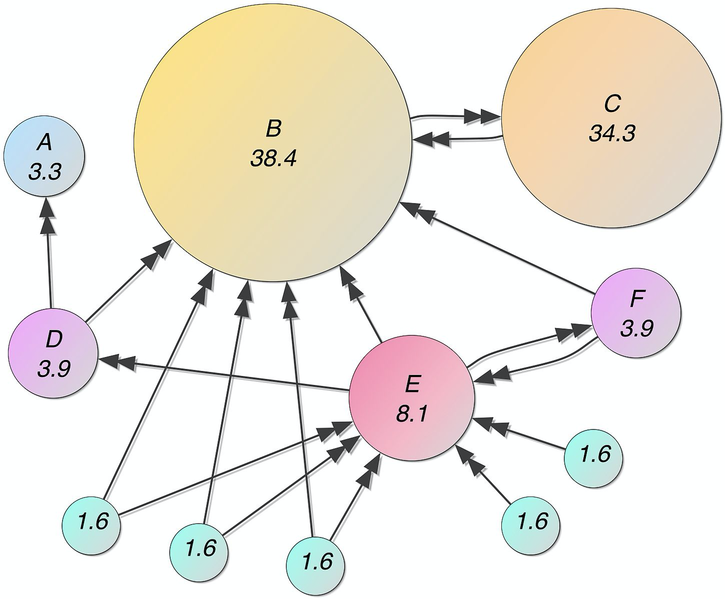
\includegraphics[width=2.5in]{images/fig3.jpeg}
    \caption{A simple illustration of PageRank, where each circle represents a web page and each arrow represents a hyperlink. The size of each circle represents the importance of each web page.}
    \label{fig3}
\end{figure}

A web page's PageRank is created by all World Wide Web pages as nodes and hyperlinks as edge, as Fig.2 shows. The PageRank value indicates the importance of a web page, aiming to measure the relative importance of each web page based on its parent web page's importance, namely the PageRank of all pages linking to it. And it is calculated recursively in the implementation of the algorithm. Besides, a hyperlink to this web page is called ``a vote of support for this web page". For instance, a page linked to more pages will have more votes, and also higher PageRank. 

\subsection{Markov Chain}

Markov chain\footnote[1]{即马尔可夫链.}, also called discrete-time\footnote[2]{即离散时间的.} Markov chain, is named after the Russian mathematician Andrei Markov. As the basis of the PageRank algorithm, it helps determine the state of each web page. Also, Markov chain has been applied to multiple statistical models.

The Markov chain is a random process that transition from a state to another in the state space\footnote[3]{即状态空间.}. The process is ``memoryless'', which means the probability distribution of the next state could merely be determined by the current state. In other words, it is irrelevant to the previous events in the time sequence. This special property ``memoryless'' is called Markov property. 

At each step of the Markov chain, the system can change from one state to another or remain unchanged, according to the probability distribution. State changes are called transitions, while the probabilities associated with different state changes are called transition probabilities.

If the Markov chain runs for enough time, the distribution of its state will reach a stationary distribution\footnote[1]{即平稳分布.}, which remains unchanged. If the Markov chain has $n$ states, the transition matrix is $P$, and the stationary distribution vector is $\boldsymbol{\pi}$, then the equation $\boldsymbol{\pi} = \boldsymbol{\pi} P$ must be satisfied.

This means that the stationary distribution vector $\boldsymbol{\pi}$ is an eigenvector\footnote[2]{即特征向量.} of the transition matrix $P$ with an eigenvalue\footnote[3]{即特征值.} of 1. A stationary distribution has the following properties:
\begin{enumerate}
	\item [1.] $\boldsymbol{\pi_i}\geq0$, and $\sum\boldsymbol{\pi_i}=1$. Each element of a stationary distribution is non-negative and sums to 1, representing probability.
	\item [2.] $\boldsymbol{\pi} = \boldsymbol{\pi} P$. The stationary distribution vector is the eigenvector of the transition matrix with an 1 eigenvalue. If it is currently stationary, then after one step of transition, the state distribution will be still stationary.
	\item [3.] \textbf{Independent to the initial state.} Whatever the initial state is, the probability distribution will utimately reach a stationary distribution.
	\item [4.] \textbf{Uniqueness}. The stationary distribution of a Markov chain is unique.
\end{enumerate}

Stationary distribution represents the stable state of the Markov chain after a series of transitions.
It measures the frequency of occurrence for each state in the entire chain, providing each proportion of time spent in the each state.

For instance, consider the process we browse web pages on the Internet. Selecting the next web page has no connection with what we browse before but depends on the current page.
It is a finite-state, and also a randomly discrete-time process.

\subsection{PageRank Algorithm and Eigenvalues of Matrix}

The PageRank algorithm is based on the matrix and the eigenvalue. Before the PageRank algorithm was proposed, eigenvalue of the matrix are used for addressing many problems, including Edmund Landau's proposal(1895) for determining the winner of a chess tournament, Gabriel Pinski and Francis Narin's work(1976) on ranking scientific journals in scientometrics, Thomas Saaty's work(1977) on the weighted alternative choice, Bradley Love and StevenSloman's work on a cognitive model, namely the centrality algorithm.

The eigenvalue of the matrix is also used by the PageRank algorithm. In the next section, we will introduce the implementation of PageRank algorithm in detail.

\section{Main Method and Theory}

\subsection{Foundational principles}

The primary implementation of the PageRank algorithm is based on the matrix operation.
Initially, we assume that there are $n$ web pages on the Internet. We can define an $n \times n$ hyperlink matrix $P$ as follows: If web page $i$ has $k (k > 0)$ hyperlinks pointing to other web pages, and if there is a hyperlink from $i$ to $j$, then $P_{ij} = 1/k$. Otherwise, $P_{ij} = 0$.

\begin{equation}
	\label{eq:1}
	Pij = 
	\begin{cases}
		\frac{1}{k} & \text{if there is a hyperlink from $i$ to $j$.} \\
		0 & \text{otherwise.}
	\end{cases}
\end{equation}

Then we can acquire the hyperlink matrix $P$ of the web pages, which is also the graph of the hyperlinked web pages.
To ensure connectivity in this graph, we assume that visitors browse randomly any web page at a certain probability. Therefore, it can be defined as stationary distribution of a Markov chain. And its state space is the set of all web pages. The transition matrix is:
\begin{equation}
	\label{eq:2}
	\widetilde{P} = cP + \frac{(1 - c)}{n}E
\end{equation}

In this equation, $E$ is a matrix that all elements equal to 1, $n$ is the number of web pages, and \(c (c \in (0,1))\) is a special parameter called \textbf{damping factor}\footnote[1]{即阻尼系数,后文会介绍到.}. It represents the probability that a vistor will not finish browsing the current web page, commonly set to $0.85$\cite{ref4}.

Since the matrix $\widetilde{P}$ is a random matrix, nonperiodic\footnote[2]{即非周期性的.}, and irreducible\footnote[3]{即不可约的.}. According to the Markov chains\cite{ref5}, a unique stationary distribution vector π exists, which is an eigenvector of the transition matrix $\widetilde{P}$ with an eigenvalue of $1$\cite{ref6}. 

\begin{equation}
	\label{eq:3}
	\pi \widetilde{P} = \pi , \pi e = 1
\end{equation}

In these equations, e is a column vector with all elements equal to 1. 

A vector π satisfying equation(3) is called the \textbf{PageRank vector}. For instance, if a visitor keeps browsing a web page with probability $c$, and jumps to a random page with probability $1 - c$, then $\pi_i$ can be understood as the stationary probability of the visitor browsing the web page $i$.

Ultimately, each value of the PageRank vector represents the PageRank value of each web page. 

Besides, the PageRank values could be described using another formula.

\begin{equation}
	\label{eq:4}
	\text{PR}(A) = \frac{1 - c}{n} + c \sum_{i} \frac{\text{PR}(T_i)}{L(T_i)}
\end{equation}

In this equation, $A$ is the web page we manage to calculate the PageRank value,  $\text{PR}(T_i)$ is the PageRank value of other web page $i$ with a hyperlink pointing to $A$, and $L(T_i)$ indicates the number of hyperlinks from other web page $i$  to any other web page $j$ (See the value $k$ in Equation (1)). It is obvious that Equations (2) and (3) are the matrix form of Equation (4).

\subsection{Overview of calculating methods}

In last subsection, we describe the principles of the PageRank algorithm. In this subsection, we will introduce its calculating methods.

PageRank can be calculated by iterative method or algebraic method\footnote[1]{即代数法.}. 

The iterative method is also called power iteration. Both the two methods include the same mathematical operations. 

In the algebraic method, PageRank values are calculated by constructing and solving a group of linear equations\footnote[2]{即线性方程组.} that describes the relationships of web pages, which requires constructing a very large matrix. Solving the system of equations is much more difficult and complex, even for computers.

But for the iterative method, it could acquire final solution by several iterations. The basic idea is to use the Equation (4) to calculate the PageRank value of the web page through iterations. By multiple iterations, the PageRank values gradually verge\footnote[3]{即趋于.} to stability. This method's code is also easier to be written. Therefore, we mainly describe the iterative method in next subsection. 

\subsection{Iterative method}

We use $PR(x, i)$ to represent the PageRank value of the web page $x$ at the $i$ iteration. At $i = 0$, we need to initialize the PageRank values for each web page.

\begin{equation}
	\label{eq:5}
	PR(P_i, 0) = \frac{1}{n}
\end{equation}

According to Equation (4), we should iteratively calculate the PageRank values by the following formula:

\begin{equation}
	\label{eq:6}
	PR(P_i, i+1) = \frac{(1 - c)}{n} + c \sum_{i} \frac{PR(P_j, i)}{L(P_i)}
\end{equation}

Besides, we know that Equation (4) can be shown in matrix form by Equation (2) and Equation (3). As a result, we can represent Equation (6) in matrix form:

\begin{equation}
	\label{eq:7}
	\pi_{i+1} = \pi_i \cdot \widetilde{P} = cP\pi_i + \frac{1 - c}{n} e
\end{equation}

According to Equation (6) or Equation (7), it can achieve stability through iterations with the condition:

\begin{equation}
	\label{eq:8}
	|PR(P_i, i+1) - PR(P_i, i)| < \varepsilon
\end{equation}
 
In this equation, \(\varepsilon\) is a very small value. At this time, the PageRank values could be considered as the final PageRank values for the web pages.

\subsection{Improved iterative method}

In the iterative method, calculating the PageRank values of all web pages still needs to conduct multiple complex matrix operation. This is a resource-consuming and time-consuming process. In this subsection, we will introduce a state-of-the-art iterative method, called the power iterative method, to reduce the complexity of the algorithm.

We assume that the hyperlink matrix is $P$, and the vector $\pi$ is the stationary distribution vector, which satisfies Equation (3). We get: 

\begin{equation}
	\label{eq:9}
	\pi = (cP + \frac{1 - c}{n}E)\pi = \widetilde{P}\pi
\end{equation}

It shows that $\pi$ is an eigenvector of the matrix $\widetilde{P}$.

Then, we could calculate starting from vector $x(0)$, repeatedly calculate with the matrix $\widetilde{P}$: 

\begin{equation}
	\label{eq:10}
	x(t+1) = \widetilde{P}x(t)
\end{equation}

until:

\begin{equation}
	\label{eq:11}
	|x(t+1) - x(t)| < \varepsilon
\end{equation}

At this time, the vector $x(t)$ represents the PageRank vector $\pi$.

\subsection{Code implementation}

In this subsection, we will introduce the code implementation of the PageRank algorithm. The code is shown in Algorithm \ref{alg:pagerank}.

\begin{algorithm}
	\caption{Power Iteration for PageRank algorithm}
	\label{alg:pagerank}
	\begin{algorithmic}[1]
	
	\REQUIRE Hyperlinks matrix $P$, Number of iterations $num$, Damping factor $c$, PageRank vector $v$
	
	\STATE $P \gets P^\top$ \COMMENT{Transpose $P$}
	\STATE $N \gets$ Number of columns in $P$
	\STATE $v \gets \frac{1}{N} \cdot \mathbf{1}_N$ \COMMENT{Initialize PageRank vector with $\frac{1}{N}$}
	\STATE $P_{\text{hat}} \gets c \cdot P + (1 - c) / N$ \COMMENT{Create hyperlinks matrix with damping factor}

	\COMMENT{Iteration for $num$ times}
	\FOR{$i \gets 1$ \TO $num$}
		\STATE $v \gets P_{\text{hat}} \cdot v$ \COMMENT{Matrix multiplies vector}
	\ENDFOR
	
	\RETURN $v$
	
	\end{algorithmic}
\end{algorithm}

In this algorithm, the parameter P represents the hyperlink matrix P, the parameter num represents the number of iterations, and the parameter c represents the damping factor c. The parameter v represents the PageRank vector.

\section{Experiment and results}

In this section, we will analyze the PageRank algorithm by demonstrating an example. Besides, we will test the damping factor that significantly affects PageRank.

\subsection{Factors that affect PageRank}

Consider a simple network consisting of four web pages, shown in Fig.3.

\begin{figure}[h]
	\centering
	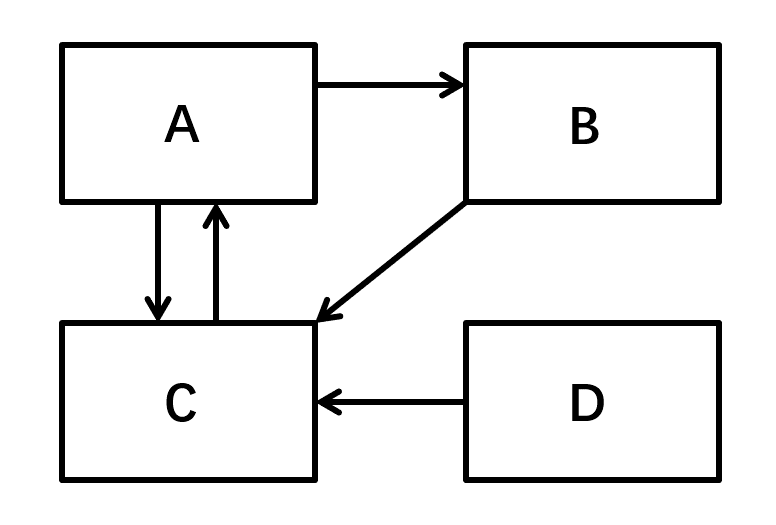
\includegraphics[width=2.5in]{images/fig5.png}
	\caption{A simple network consisting of four web pages.}
	\label{fig4}
\end{figure}

We could get its hyperlink matrix $P$ by using Equation (1):
\begin{equation}
	\label{eq:12}
	P = \begin{bmatrix}
		0 & \frac{1}{2} & \frac{1}{2} & 0 \\
		0 & 0 & 1 & 0 \\
		1 & 0 & 0 & 0 \\
		0 & 0 & 1 & 0 \\
		\end{bmatrix}
\end{equation}

We assumes that the damping factor $c$ is $0.85$, as Google commonly uses, and then calculate its transition matrix.

\begin{equation}
	\label{eq:13}
	\widetilde{P} = \begin{bmatrix}
		0.0375 & 0.4625 & 0.4625 & 0.0375 \\
		0.0375 & 0.0375 & 0.8875 & 0.0375 \\
		0.8875 & 0.0375 & 0.0375 & 0.0375 \\
		0.0375 & 0.0375 & 0.8875 & 0.0375 \\
		\end{bmatrix}
\end{equation}

In this matrix, $\widetilde{P}_{ij}$ represents the probability that visitors choose to jump from page $i$ to page $j$.

We assume that $t$ is the iteration number. When $t = 0$, the initial PageRank values for each web page are set to 0.25.

\begin{equation}
	\label{eq:14}
	x(0) = \begin{bmatrix}
		0.25 \\
		0.25 \\
		0.25 \\
		0.25 \\
		\end{bmatrix}
\end{equation}

After the first iteration, we get:

\begin{equation}
	\label{eq:15}
	x(1) = \begin{bmatrix}
		0.25 \\
		0.14375 \\
		0.56875 \\
		0.0375 \\
		\end{bmatrix}
\end{equation}

We could draw the transition of the PageRank values from $t = 0$ to $t = 1$ by graph:

\begin{figure}[h]
	\centering
	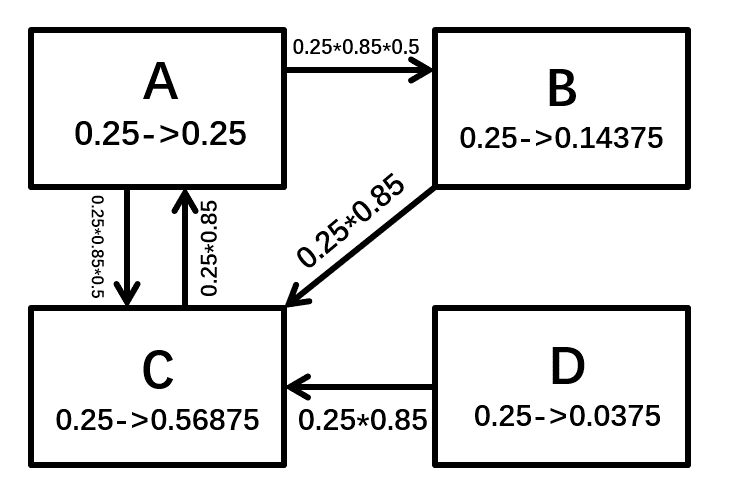
\includegraphics[width=2.5in]{images/fig6.png}
	\caption{The transition of the PageRank values from $t = 0$ to $t = 1$.}
	\label{fig6}
\end{figure}

In each iteration, the PageRank value of the current web page multiplies the damping factor c, so that it evenly transferred to the web page that need to be calculated. 

As iterations continue, the PageRank values tend to be stable:

\begin{equation}
	\label{eq:16}
	x(1) = \begin{bmatrix}
		0.37252685 \\
		0.19582391 \\
		0.39414924 \\
		0.0375 \\
		\end{bmatrix}
\end{equation}

We could also draw the line chart to describe the changes in PageRank values during the iteration process:

%TODO需要重新画图
\begin{figure}[h]
	\centering
	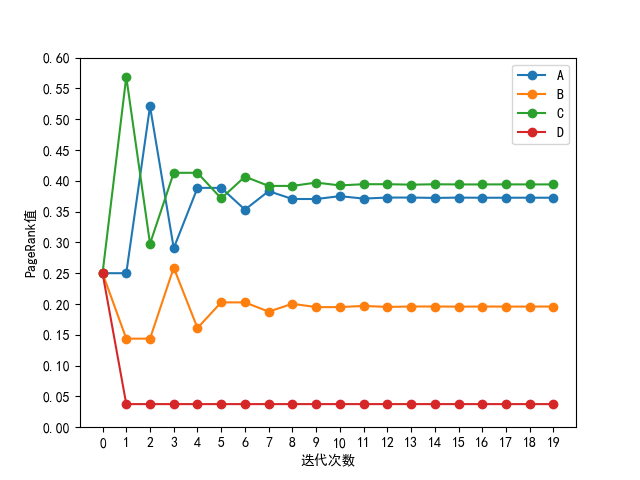
\includegraphics[width=2.5in]{images/fig7.png}
	\caption{Changes in PageRank values during the iteration process}
	\label{fig7}
\end{figure}

The ultimate order of web pages is $C, A, B, D$. 

We could conclude that the PageRank value of a web page is related to both the number of web pages pointing to it and the PageRank values of these pages. To explain it, web page $C$ has the highest number of links, leading to the highest PageRank value. $A$ and $B$ have an equal number of links, but due to the higher PageRank value of $C$, which points to $A$, $A$'s PageRank value is higher than $B$. There is no page points to page $D$, so that its PageRank value is the lowest.

\subsection{Damping factor}

The damping factor is a significant parameter that could affect the PageRank value. In this section, we will analyze the impact of the damping factor on the PageRank value.

Still consider the simple network shown in Fig.3.

We can draw a line chart to illustrate the variation of PageRank values for each webpage with different damping factor $c (c \in (0,1))$ values in Fig.6.

\begin{figure}[h]
	\centering
	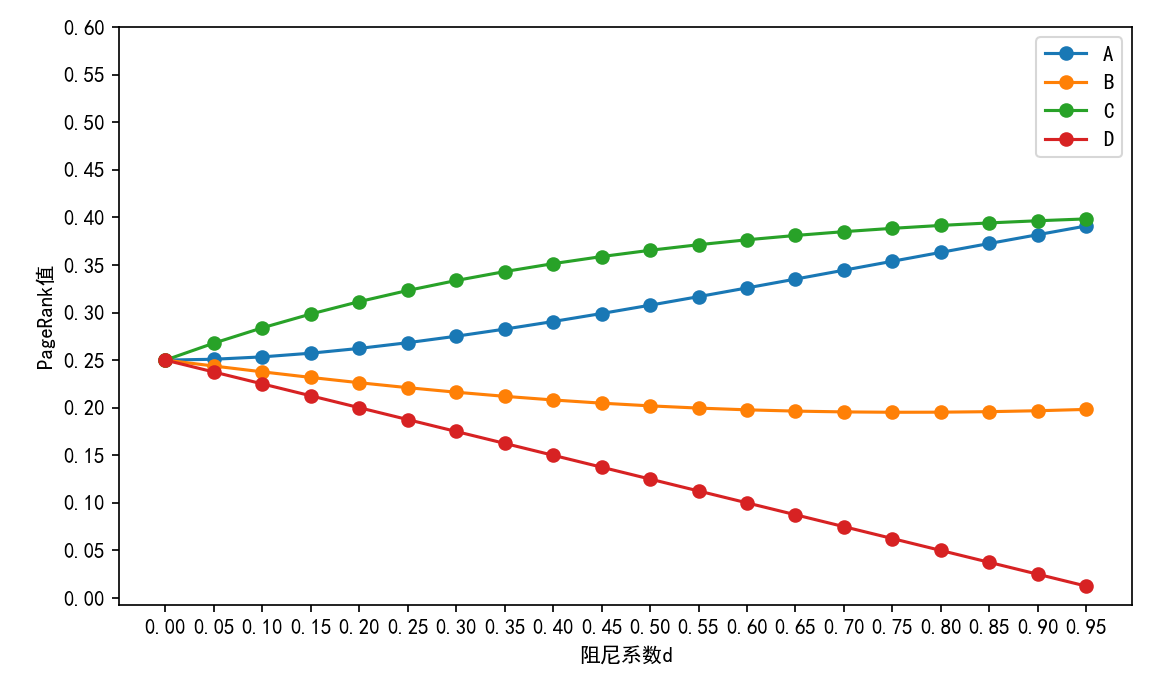
\includegraphics[width=2.5in]{images/fig8.png}
	\caption{The variation of PageRank values for each webpage with different damping factor $c$ values.}
	\label{fig8}
\end{figure}

It is obvious that the PageRank values of web pages differs significantly with a larger damping factor $c$, making it easier to distinguish the 'quality' of web pages. 

Then, we consider a simpler network, as shown in Fig.7.

\begin{figure}[h]
	\centering
	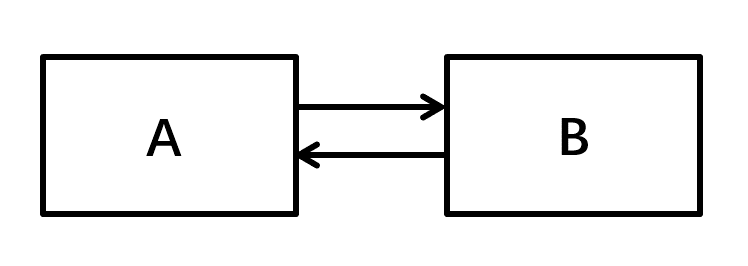
\includegraphics[width=2.5in]{images/fig9.png}
	\caption{A simpler network consisting of two web pages.}
	\label{fig9}
\end{figure}

Its line chart of PageRank values with different damping factor $c$ values could be drawn in Fig.8.

\begin{figure}[h]
	\centering
	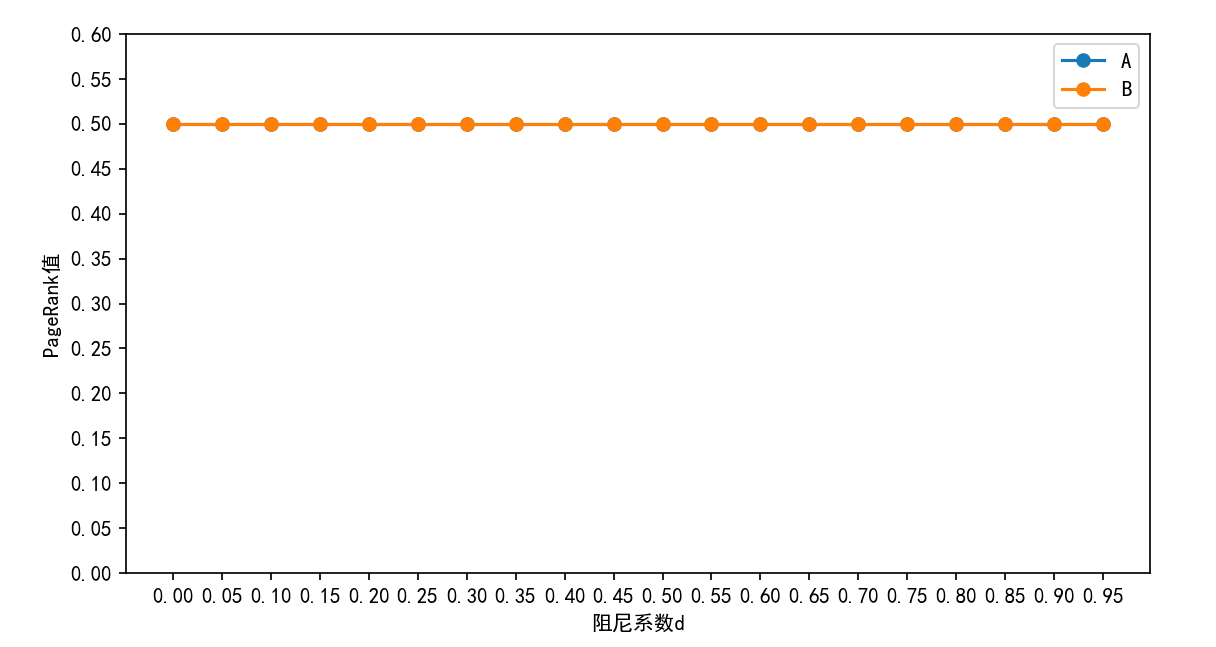
\includegraphics[width=2.5in]{images/fig10.png}
	\caption{The line chart of PageRank values with different damping factor $c$ values.}
	\label{fig10}
\end{figure}

In this case, the PageRank values of web pages are almost the same with different damping factor $c$ values.

At last, we consider another network, as shown in Fig.9.

\begin{figure}[h]
	\centering
	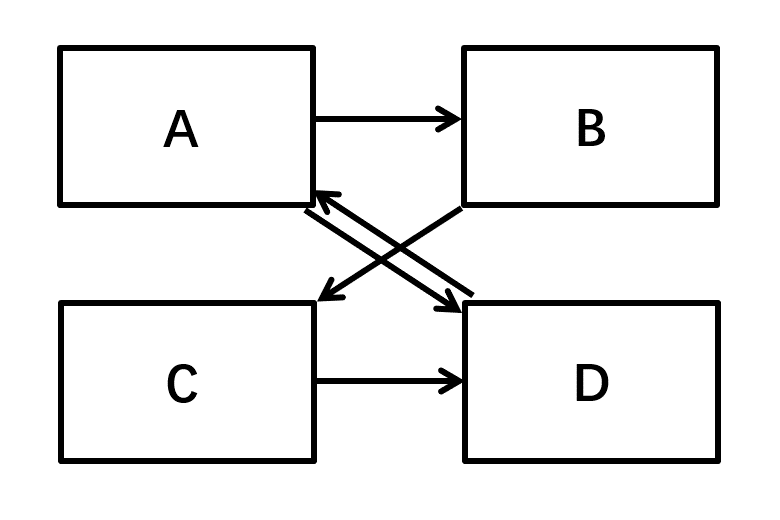
\includegraphics[width=2.5in]{images/fig11.png}
	\caption{The line chart of PageRank values with different damping factor $c$ values.}
	\label{fig11}
\end{figure}

Its line chart of PageRank values with different damping factor $c$ values could be drawn in Fig.9.

\begin{figure}[h]
	\centering
	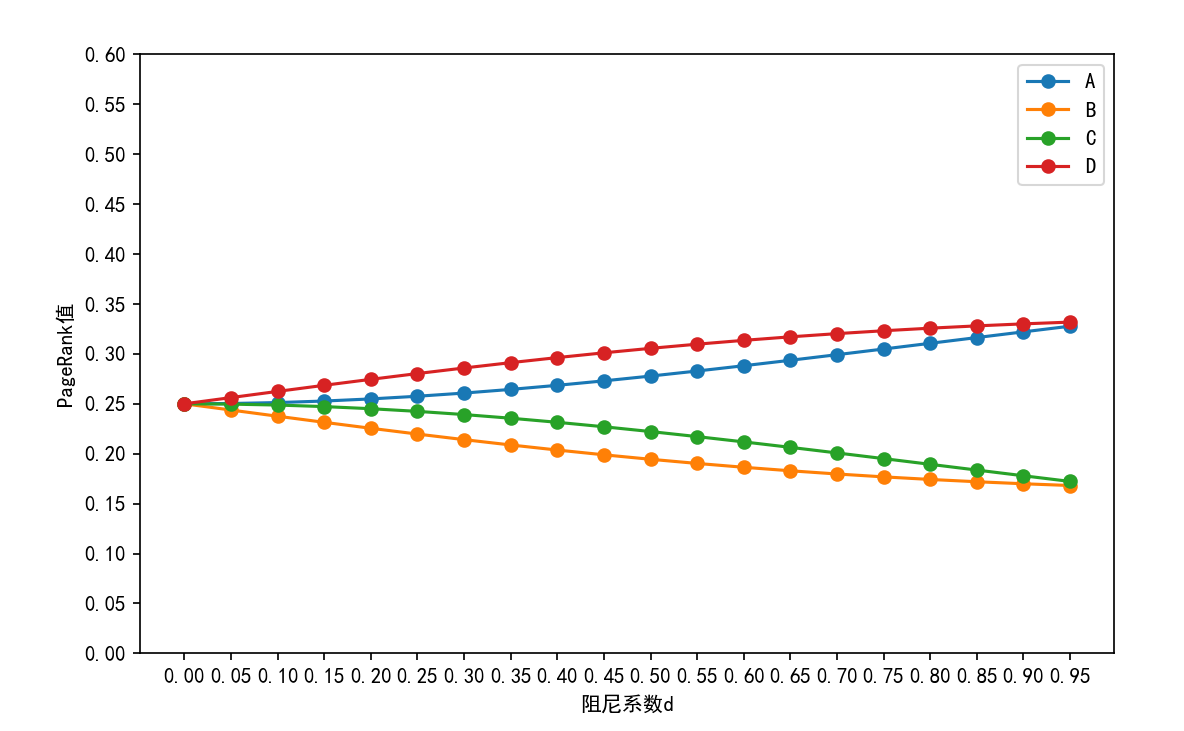
\includegraphics[width=2.5in]{images/fig12.png}
	\caption{The line chart of PageRank values with different damping factor $c$ values.}
	\label{fig12}
\end{figure}

In this case, the damping factor $c$ in the middle is appropriate. If we choose the $c$ to be too small or too large, it may be hard to differentiate two pairs of web pages.

To sum up, the change of the damping factor $c$ will affect different web pages' PageRank value in different networks. The degree of this affect depends on the structure of network. 

According to the assumption of the Markov chain and general habbit of browsing the Internet, it is assumed that the damping factor closer to 1 causes appropriate results. However, in networks similar to the Network shown in Fig.9, when the damping factor is too close to 1, it is hard to differentiate two pairs of web pages. Therefore, the damping factor of $0.85$ may be the most appropriate value after a large number of experiments by Google.

\section{Discussion on potential enhancements}

In this section, we will discuss the flaws of the PageRank algorithm and enhancements.

\subsection{Flaws}

Although PageRank is a widely used web page ranking algorithm, it has several flaws.

The biggest flaw is called ``uniform access assumption''\footnote[1]{即均匀访问假设.}. It assumes that users have an equal probability to access all web pages. Apparently, it is not true. Users' hobbies and social areas may affect this possibility.

Except the ``uniform access assumption'', there are other flaws:
\begin{itemize}
	\item \textbf{Handling a large number of web pages is time-consuming}. The PageRank algorithm needs to calculate the PageRank value of each web page, which is time-consuming when the number of web pages is too large.
	\item \textbf{Vulnerability to spam links is a serious problem}. Spam links\footnote[1]{即垃圾链接.} are those that exist on low-quality web pages. Their presence can influence the entire page ranking system. In actual situations, PageRank is susceptible to be exploited, causing the fake search results. For example, some web page owners may deliberately create a large number of web pages so as to point to their own web pages, which will increase the PageRank of their web pages. Also, relevant research tends to focus on some web pages' PageRank affected by errors. In order to solve this problem, Google set up a new attribute ``nofollow'' for all web links, which allows web-masters and blogger to create some links that are not important, so that these links do not serve as the ``vote''.
	\item \textbf{Its difficulty in handling dynamic web pages}. If the content of a web page changes frequently, the PageRank algorithm may not be able to reflect these changes in a timely manner. For example, a news websites publishes a large number of news every day. If the search engine calculates its PageRank value once, the importance of these news will not be shown in the ranking in time.
	\item \textbf{PageRank also suffers from data sparsity and lack of topics}. In some cases, the PageRank may overlook some important web pages due to a lack of links to web pages relevant to the search topic. In addition, because PageRank only considers link structure but ignores the topic and content of web pages, it may not provide the best results in some specific areas.
\end{itemize}

\subsection{Way of Enhancements}

In last subsection, we discussed the flaws of the PageRank algorithm. Some of them could be solved by the specific methods in this subsection.

\subsubsection{Matrix Decomposition}

The number of web pages is extremely large on the Internet. How to calculate the PageRank value of each page is a key issue. One way to solve the issue is to do this is to explore the specific properties of the hyperlink matrix $P$.

Consider the hyperlink matrix $P$ of the following form:

\begin{equation}
	\label{eq:114514}
	P=
	\begin{bmatrix}
		P_1    & \cdots & 0      \\
		\vdots & \ddots & \vdots \\
		0      & \cdots & P_N
	\end{bmatrix}
\end{equation}

The block $ P_I (I = 1, \ldots, N)$ on the diagonal represents the link within group $I$. We use $n_I$ to represent the number of pages within Group $I$. Each block $I$ does not communicate with the outside world, but there may be a complex relation inside.

Next, we consider the transition matrix of the hyperlink matrix \eqref{eq:114514}:

\begin{equation}
	\label{eq:114515}
	\widetilde{P} = cP  + (1-c)(1/n)E
\end{equation}

We assume that the vector $\boldsymbol{\pi}$ is the PageRank vector of the transition matrix $\widetilde{P}$, which satisfies $\boldsymbol{\pi}\widetilde{P}=\boldsymbol{\pi}, \boldsymbol{\pi e}=1$. In addition, we could define the perturbation matrix\footnote[1]{即摄动矩阵.} of block $I$.

\begin{equation}
	\widetilde{P_I}
	=cP_I + \frac{1-c}{n_I}E
\end{equation}
Next, we let the vector $\boldsymbol{\pi}_I$ be PageRank vector of $\widetilde{P}_I$, and make
\begin{equation}
	\boldsymbol{\pi}_I\widetilde{P}_I = \boldsymbol{\pi}_I, \boldsymbol{\pi}_I\boldsymbol{e}=1
\end{equation}

We can acquire the following formula by proof:

\begin{equation}
	\label{eq:4444}
	\boldsymbol{\pi}=\frac{1}{n}(n_1\boldsymbol{\pi}_1,  n_2\boldsymbol{\pi}_2,\ldots,n_N\boldsymbol{\pi}_N)
\end{equation}

\begin{proof}


	define:
	\begin{equation}
		\widetilde{E}=
		\begin{bmatrix}
			\frac{1}{n_1}E & \cdots & 0              \\
			\vdots         & \ddots & \vdots         \\
			0              & \cdots & \frac{1}{n_N}E
		\end{bmatrix}
	\end{equation}

	To the $\boldsymbol{\pi}$ in \eqref{eq:4444}
	\begin{equation}
		\begin{aligned}
			\boldsymbol{\pi}\widetilde{P} & = \boldsymbol{\pi}[cP+(1-c)\overline{E}                                                                   \\
			                              & -(1-c)\overline{E}+(1-c)(1/n)E]                                                                           \\
			                              & =\boldsymbol{\pi}[cP+(1-c)\overline{E}]                                                                   \\
			                              & +\boldsymbol{\pi}[(1-c)\overline{E}+(1-c)(1/n)E]                                                          \\
			                              & =(\frac{n_1}{n}\boldsymbol{\pi}_1\widetilde{P_1},\ldots,\frac{n_N}{n}\boldsymbol{\pi}_N\widetilde{P_N})   \\
			                              & +(1-c)(1/n)e^T-(1-c)(1/n)e^T                                                                              \\
			                              & =\frac{1}{n}(n_1\boldsymbol{\pi}_1,  n_2\boldsymbol{\pi}_2,\ldots,n_N\boldsymbol{\pi}_N) \\
			                              & =\boldsymbol{\pi}
		\end{aligned}
	\end{equation}

\end{proof}
Since $\widetilde{P}$ 's PageRank vector is unique, $\boldsymbol{\pi}$ is $\widetilde{P}$ 's PageRank vector.

This decomposition\footnote[1]{即矩阵分解.} property can also be expressed by the following formula:
\begin{equation}
	\boldsymbol{\pi}=
	\frac{1-c}{n}e^T[1-cP]^{-1}
\end{equation}

If the hyperlink matrix is extremely sparse, and the time complexity\footnote[2]{即时间复杂度.} is close to linear in the number of pages. Since we have decomposed the hyperlink matrix, we can process each part independently and store different parts of the PageRank vector in different databases\footnote[1]{即数据库.} to save time and space.

\subsubsection{Topic-sensitive PageRank}

The Topic-sensitive PageRank is an extension of the PageRank algorithm.

It is designed to improve the accuracy of search results. Unlike the traditional PageRank, it do not considers the global importance of the page anymore, but ranks web pages based on the importance of a topic, which is more effective for search results that require a specific topic.

The main idea of Topic-sensitive PageRank is to build multiple PageRank vectors based on a topic. We use them to calculate the weight of a web page. 

In a regular keyword search query, we can use the topic of the query keyword to calculate a web page's topic-sensitive PageRank score Number. 

In contextual\footnote[2]{即上下文搜索.} search, the topic of the query context can be used to calculate the topic-sensitive PageRank score for the web page. By using these linear combinations of topic-biased PageRank vectors, it is possible to generate a context-specific page importance score at query time.This may generate more accurate ranking results than using a single PageRank vector.

\begin{figure*}[!t]
	\centering
	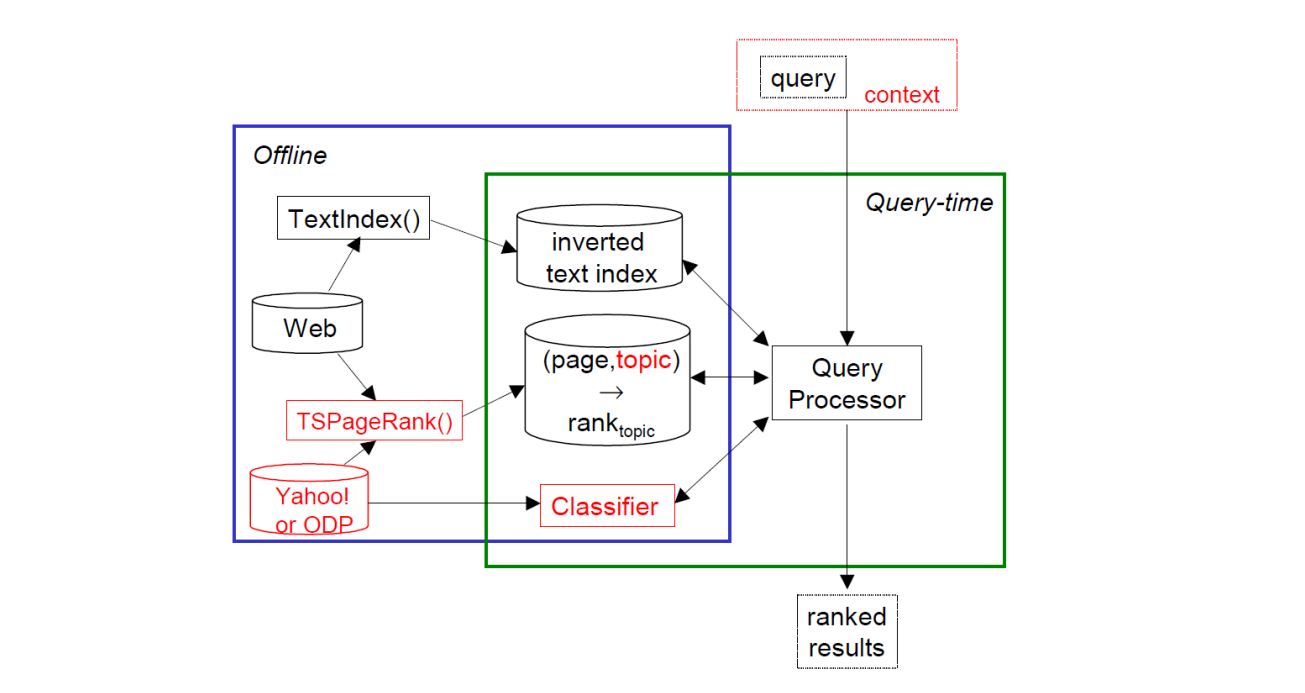
\includegraphics[width=\textwidth]{images/fig4.png}
	\caption{A system diagram that uses a topic-sensitive PageRank.}
	\label{fig5}
\end{figure*}

This topic-sensitive method can be demonstrated by the following example:\cite{ref7}
By using web crawler\footnote[3]{即网络爬虫.}, we generated 16 topic-sensitive PageRank vectors by using URLs from OpenDirectoryProject\footnote[4]{ODP, a web directory with more than 2.5 million URLs.}. 
At query time, we calculate the similarity of between the query and each topic. 
Then, instead of using a PageRank vector, we use topic-sensitive vectors, weighted using the similarity. 
By using a group of rank vectors, we can more accurately identify the most important pages relevant to a particular query or query context. 
Since some of calculations are processed offline, the query time cost is no higher than the normal PageRank.

\subsubsection{Sparse Matrix Enhancement}

A sparse matrix or sparse array is a matrix where most of the elements are zero. 
A standard to judge it is that the number of non-zero elements is roughly equal to the number of rows or columns. By contrast, if most of the elements are non-zero, the matrix is considered dense.

There is an example of sparse matrix.

\begin{equation}
	A_{6\times 7}=
	\begin{bmatrix}
		0&0&1&0&0&0&0\\
		0&2&0&0&0&0&0\\
		3&0&0&0&0&0&0\\
		0&0&0&0&6&0&0\\
		0&0&0&0&0&7&4
	\end{bmatrix}
\end{equation}

The most calculation-intensive part of the PageRank algorithm is to calculate the link weight between web pages that involves summing\footnote[1]{即求和.} the links of each web page. 
Since the number of links for most web pages is very large, and many elements of it is zero. We can use the sparse matrix algorithm to solve the PageRank Matrix, which means we only need solve the non-zero elements.

We can use the Compressed Sparse Row (CSR) format to conduct sparse matrix optimization. 
In the CSR format, each non-zero element in the matrix saves its value, column index, and row offset. 
The row offset indicates the position of the first non-zero element in each row. 
And each row of the matrix can be represented by a single array. 
Remaining only non-zero elements to be processed, this approach can greatly reduce the calculation complexity, lowering computation time and memory consumption, also allowing the algorithm to handle larger collections of web pages.

\section{Conclusion}

As one of the most significant algorithms in the field of web searching, PageRank algorithm perform well in the current stage of the Internet. In this paper, we introduce the basic idea of PageRank algorithm, analyzing the algorithm in detail. Besides, we research the factors that affect the PageRank algorithm results, especially the damping factor, certifying the appropriateness of the damping factor $0.85$. Based on the PageRank algorithm's flaws, we introduce several effective enhancements, including matrix decomposition, the topic-sensitive PageRank, sparse matrix enhancement. For us, one persistent effort to study PageRank is that we believe it will influence the AI\footnote[1]{Artificial Intelligence.} and the future deeply. In future, the PageRank algorithm may not meet the demand of the Internet, we expect that improved PageRank algorithm will be created to solve the problem. 

\begin{thebibliography}{1}

	\bibitem{ref1}
	G. Salton and M. McGill. McGraw-Hill, {\it{Introduction to modern information retrieval }}. School of Library Science University of North Carolina Chapel Hill, North Carolina NC 27514, U.S.A., 1983. 
    \bibitem{ref2}
    G. Salton, A. Wong, C. S. Yang, {\it{A vector space model for automatic indexing}}. Association for Computing Machinery, New York, NY, United States, 1975.
	\bibitem{ref3}
	JON M. KLEINBERG, {\it{Authoritative Sources in a Hyperlinked Environment}}. Cornell University, Ithaca, New York, United States, 1999.
	\bibitem{ref4}
	Sergey Brin, Lawrence Page, {\it{The Anatomy of a Large-Scale Hypertextual Web
	Search Engine}}. Computer Science Department, Stanford University, Stanford, CA 94305, USA, 1998.
	\bibitem{ref5}
	RajeevMotwani, PrabhakarRaghavan, {\it{Randomized Algorithms.}}. Cambridge University Press, United Kingdom, 1995.
	\bibitem{ref6}
	Avrachenkov K, Litvak N, {\it{Decomposition of the google pagerank and optimallinking strategy[D].}} INRIA, 2004.
	\bibitem{ref7}
	Haveliwala T H., {\it{Topicsensitive pagerank}}, Proceedings of the 11th international conference on World Wide Web, 2002.

\end{thebibliography}

\end{document}


